\section{Eksperymenty}
Wykonaliśmy szereg testów, sprawdzających jak działa aplikacja w zależności od następujących parametrów:
\begin{itemize}
    \item liczebność populacji
    \item liczebność populacji $\lambda$
    \item liczba prostokątów w osobniku
    \item strategia krzyżowania
    \item strategia wybierania kolejnej generacji populacji
\end{itemize}

\subsection{Eksperymenty i wyniki}
W celu uzyskania możliwie jak najbardziej prawdziwych wyników dla każdego przypadku testowego, każdy eksperyment z danymi parametrami był przeprowadzony 5 razy. Wszystkie testy zostały wykonane dla obrazu na Rysunku~\ref{fig:test_image} oraz z warunkami stopu 1000 iteracji lub dokładność 99\%. 
\begin{figure}[H]
    \centering 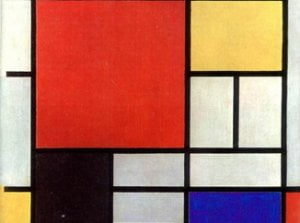
\includegraphics[width=0.5\linewidth]{img/simple_img.jpg}
    \caption{Obrazek użyty w eksperymentach}
    \label{fig:test_image}
\end{figure}
Gdy nie było to przedmiotem eksperymentu to metodą krzyżowania było uśrednianie, a metodą wybierania - wybór $\mu$ najlepszych. Wykresy są tworzonę na podstawie punktów w których zmieniała się wartość funkcji dopasowania dla najlepszego osobnika, dlatego niektóre przebiegi kończą się wcześniej. Oznacza to, że wynik się nie zmienił już do końca eksperymentu.

\subsection*{Wpływ liczebności populacji}
Test wpływu liczebności populacji został przeprowadzony dla populacji o wielkościach: 2, 10, 15, 30, 40, 50, 100, liczbie prostokątów w osobniku równej 20, wielkości populacji $\mu$ będącej 1,5 raza większej od wielkości testowanej populacji.

\begin{table}[H]
    \centering
    \begin{tabular}{|c|c|c|}
    \hline
    Liczebność populacji    & Najlepszy osobnik & Średnio najlepszy osobnik \\ \hline
    2                       & 81\%              & 75\%                      \\ \hline
    10                      & 88\%              & 80\%                      \\ \hline
    15                      & 87\%              & 80\%                      \\ \hline
    30                      & 86\%              & 78\%                      \\ \hline
    40                      & 89\%              & 84\%                      \\ \hline
    50                      & 90\%              & 89\%                      \\ \hline
    100                     & 90\%              & 86\%                      \\ \hline
    \end{tabular}
    \caption{Wyniki testów liczebności populacji}
    \label{tab:crossing}
\end{table}

Z wyników tego testu można zauważyć, że zwiększanie wielkości populacji daje lepsze wyniki. Dzieje się tak z tego powodu, że większa populacja oznacza większą różnorodność w populacji i większe prawdopodobieństwo pojawienie się osobnika optymalnego.

\begin{figure}[H]
    \centering 
    \begin{subfigure}[b]{0.49\linewidth}
        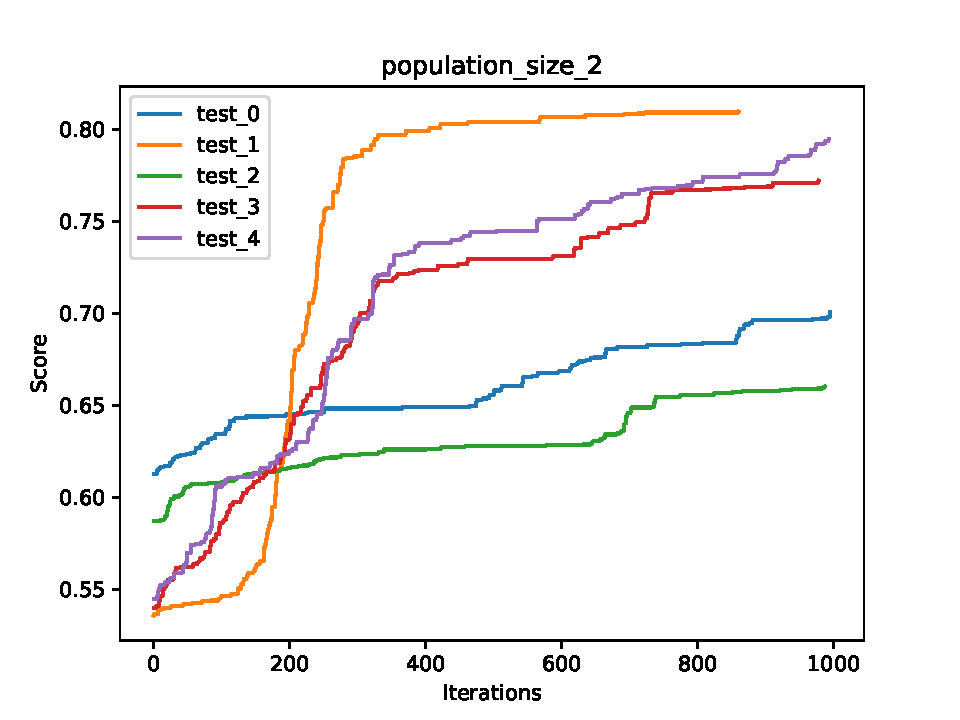
\includegraphics[width=\linewidth]{img/population_size_2.pdf}
        \caption{$\mu$ = 2}
    \end{subfigure}
    \begin{subfigure}[b]{0.49\linewidth}
        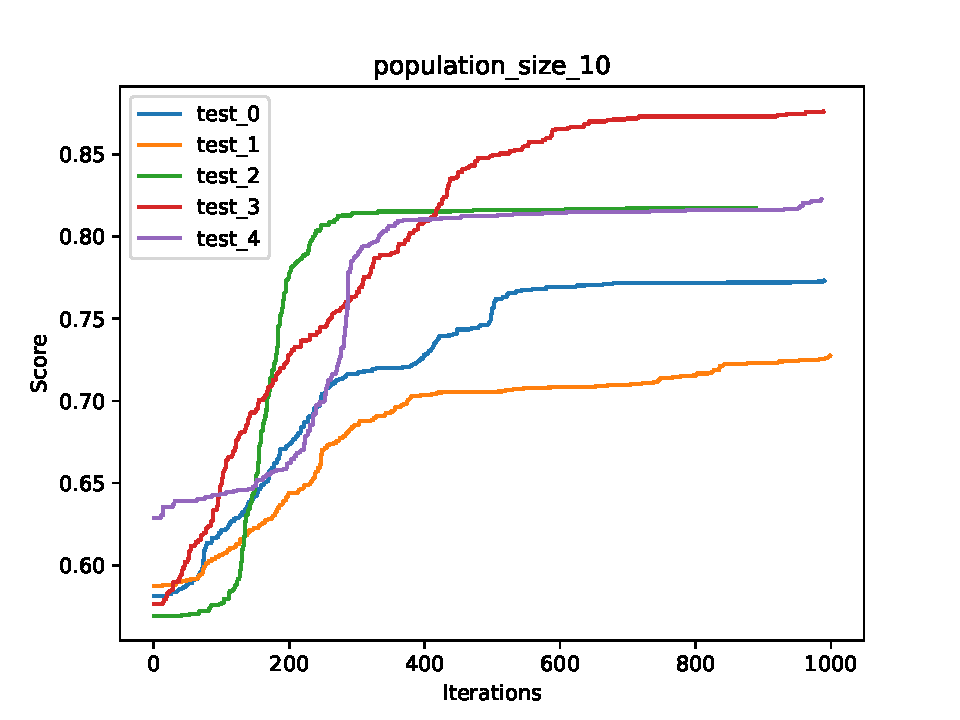
\includegraphics[width=\linewidth]{img/population_size_10.pdf}
        \caption{$\mu$ = 10}
    \end{subfigure}
    \begin{subfigure}[b]{0.49\linewidth}
        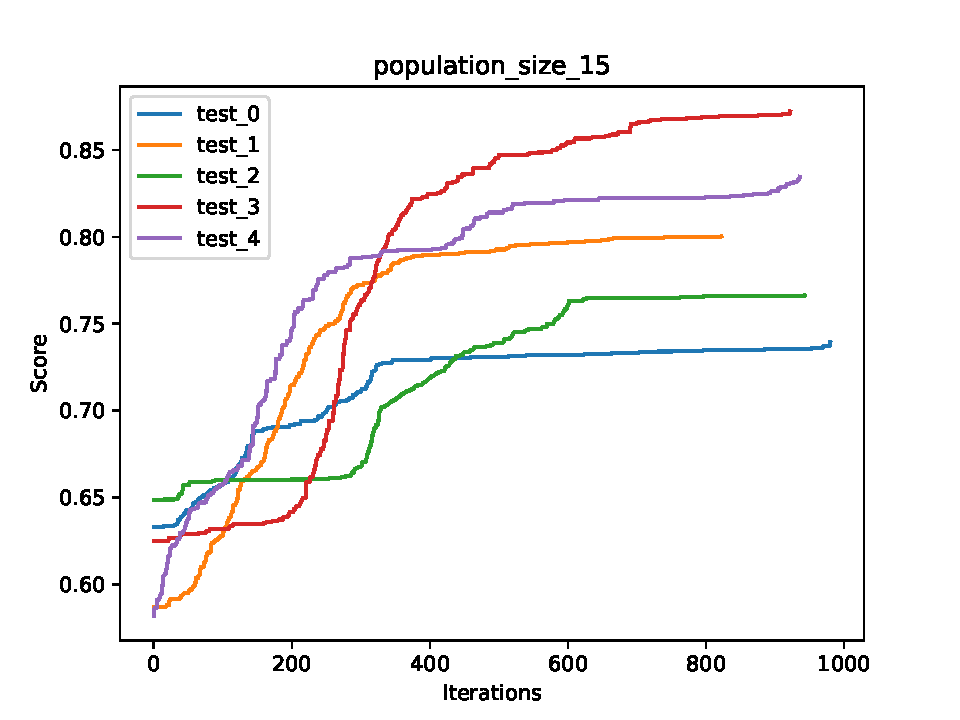
\includegraphics[width=\linewidth]{img/population_size_15.pdf}
        \caption{$\mu$ = 15}
    \end{subfigure}
    \begin{subfigure}[b]{0.49\linewidth}
        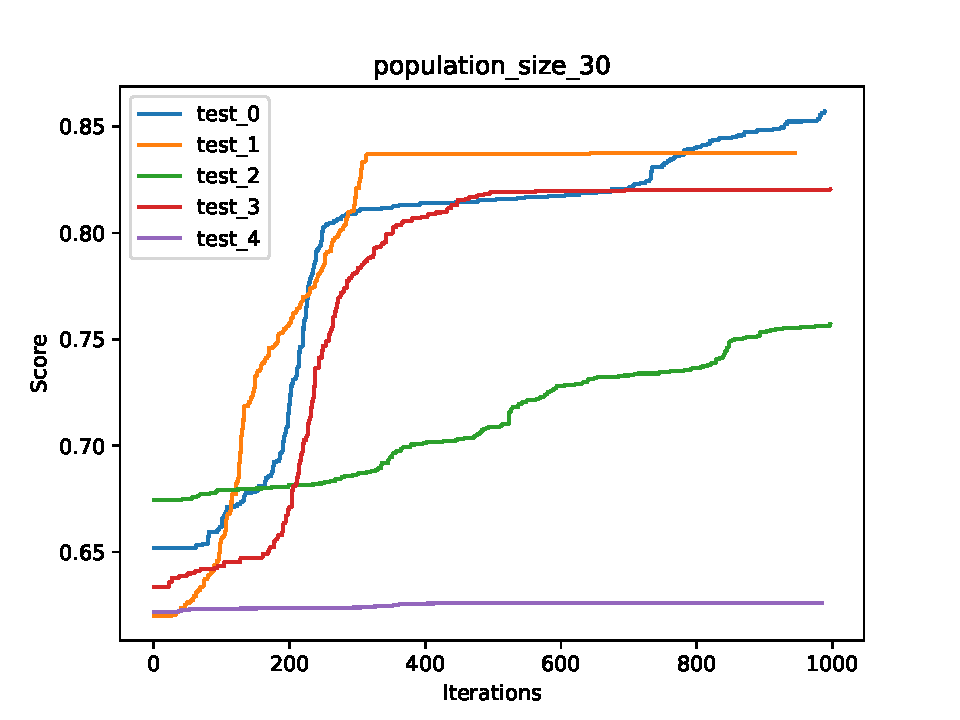
\includegraphics[width=\linewidth]{img/population_size_30.pdf}
        \caption{$\mu$ = 30}
    \end{subfigure}
    \begin{subfigure}[b]{0.49\linewidth}
        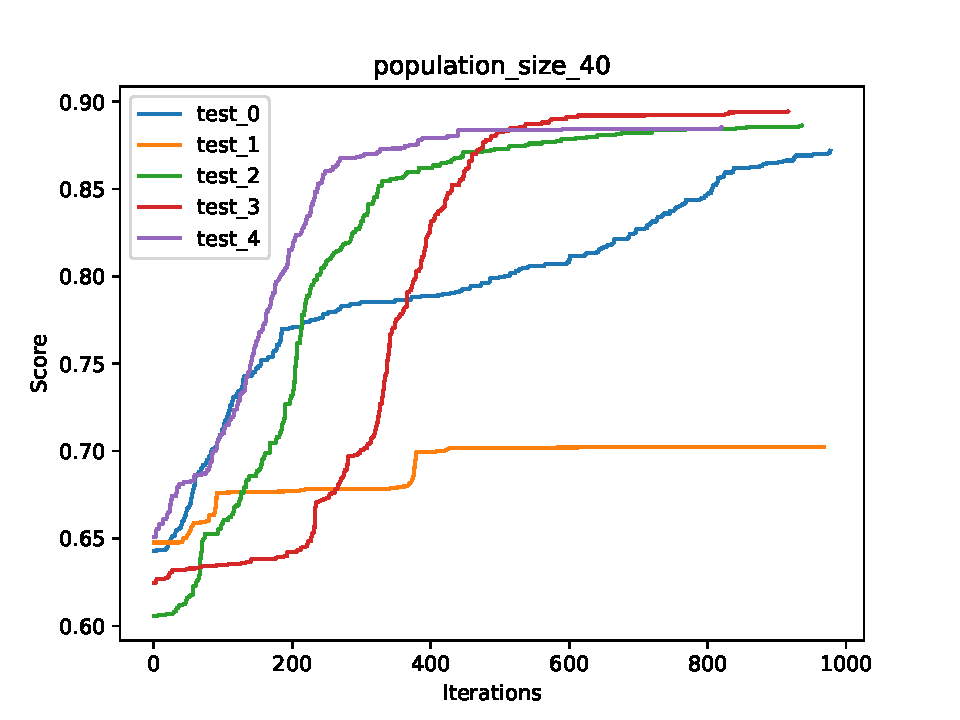
\includegraphics[width=\linewidth]{img/population_size_40.pdf}
        \caption{$\mu$ = 40}
    \end{subfigure}
    \begin{subfigure}[b]{0.49\linewidth}
        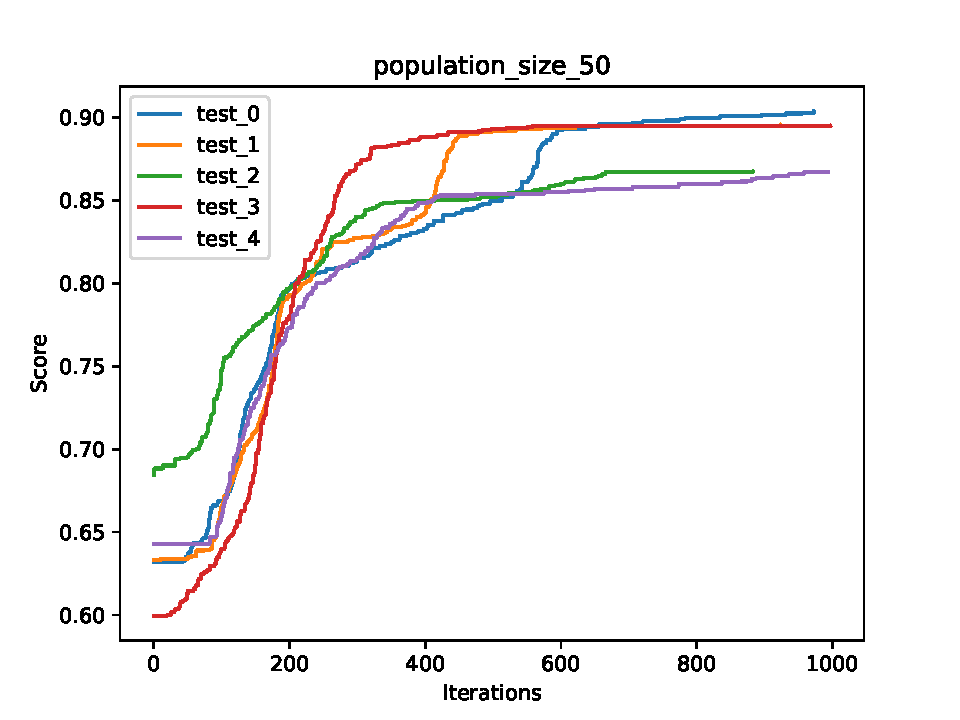
\includegraphics[width=\linewidth]{img/population_size_50.pdf}
        \caption{$\mu$ = 50}
    \end{subfigure}
    \begin{subfigure}[b]{0.49\linewidth}
        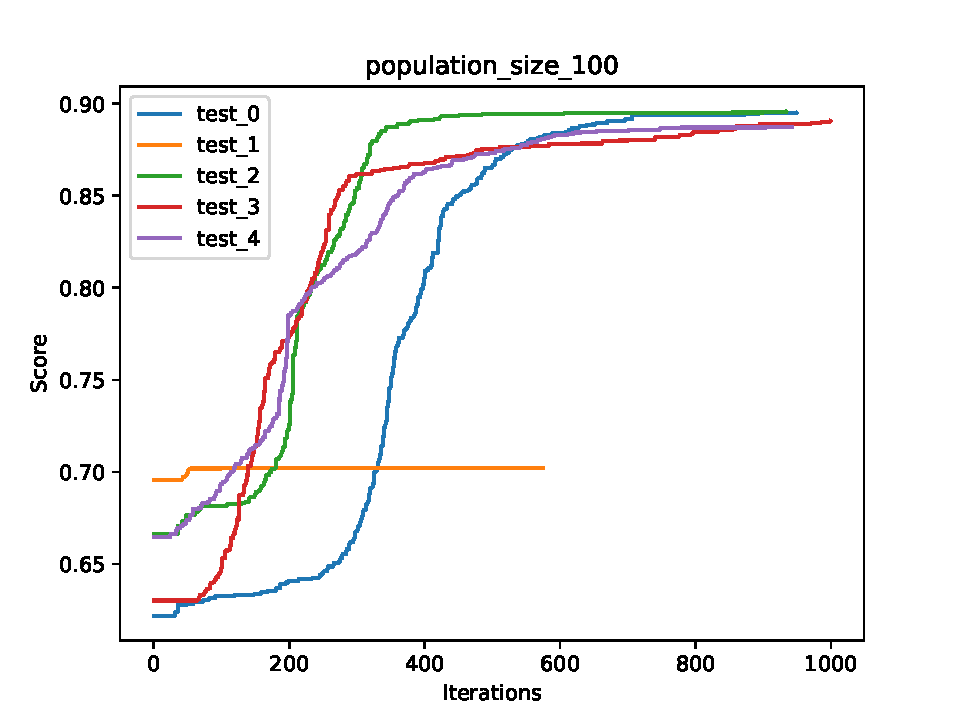
\includegraphics[width=\linewidth]{img/population_size_100.pdf}
        \caption{$\mu$ = 100}
    \end{subfigure}
    \caption{Wielkość populacji}
    \label{fig:picking}
\end{figure}

\subsection*{Wpływ liczebności populacji $\lambda$}
Test wpływu liczebności populacji $\lambda$ został przeprowadzony dla stałej wielkości populacji $\mu$ równej 40 na podstawie której kolejne przypadki testowe był obliczane za pomocą wartości procentowych: 110\%(44), 130\%(52),
150\%(60), 200\%(80), 250\%(100), 300\%(120). Liczba prostokątów w osobniku była równa 20.

\begin{figure}[H]
    \centering 
    \begin{subfigure}[b]{0.49\linewidth}
        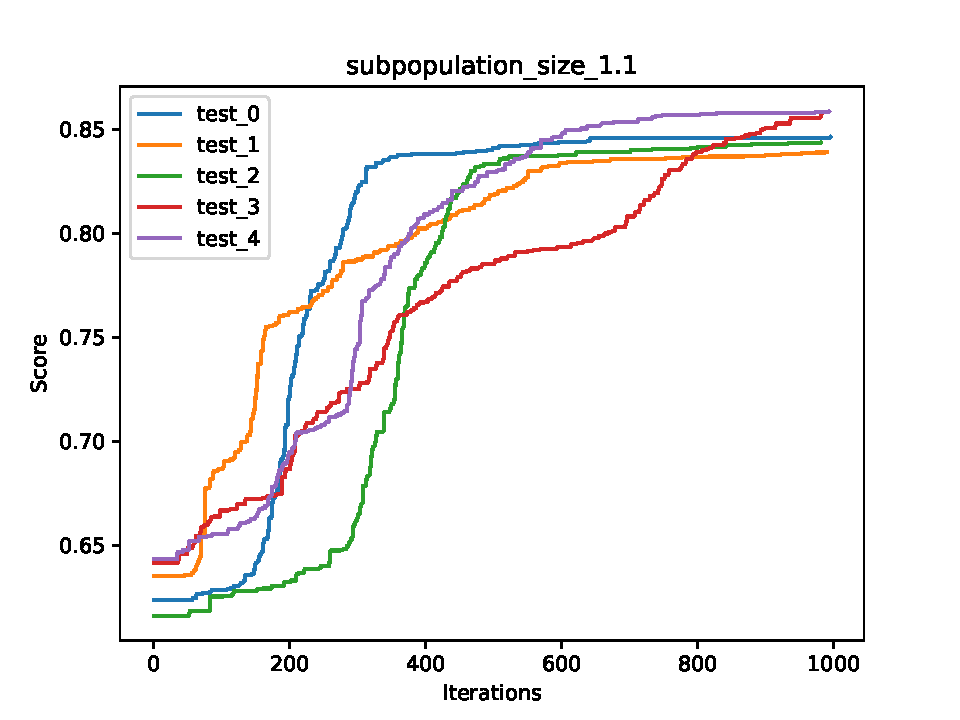
\includegraphics[width=\linewidth]{img/subpopulation_size_1.1.pdf}
        \caption{$\lambda$ = 110\%}
    \end{subfigure}
    \begin{subfigure}[b]{0.49\linewidth}
        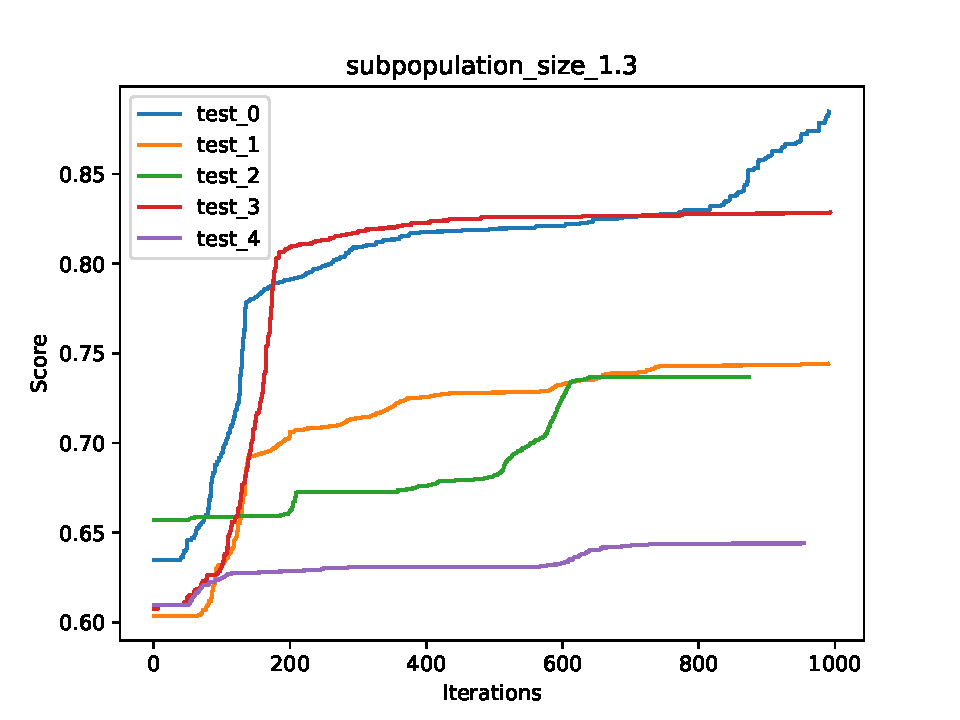
\includegraphics[width=\linewidth]{img/subpopulation_size_1.3.pdf}
        \caption{$\lambda$ = 130\%}
    \end{subfigure}
    \begin{subfigure}[b]{0.49\linewidth}
        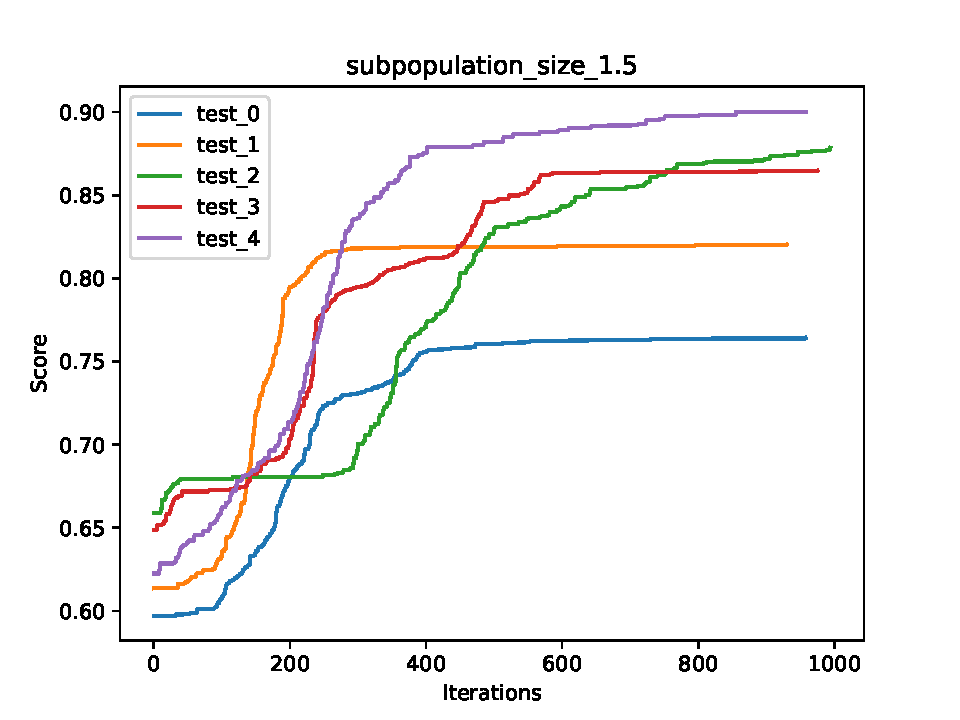
\includegraphics[width=\linewidth]{img/subpopulation_size_1.5.pdf}
        \caption{$\lambda$ = 150\%}
    \end{subfigure}
    \begin{subfigure}[b]{0.49\linewidth}
        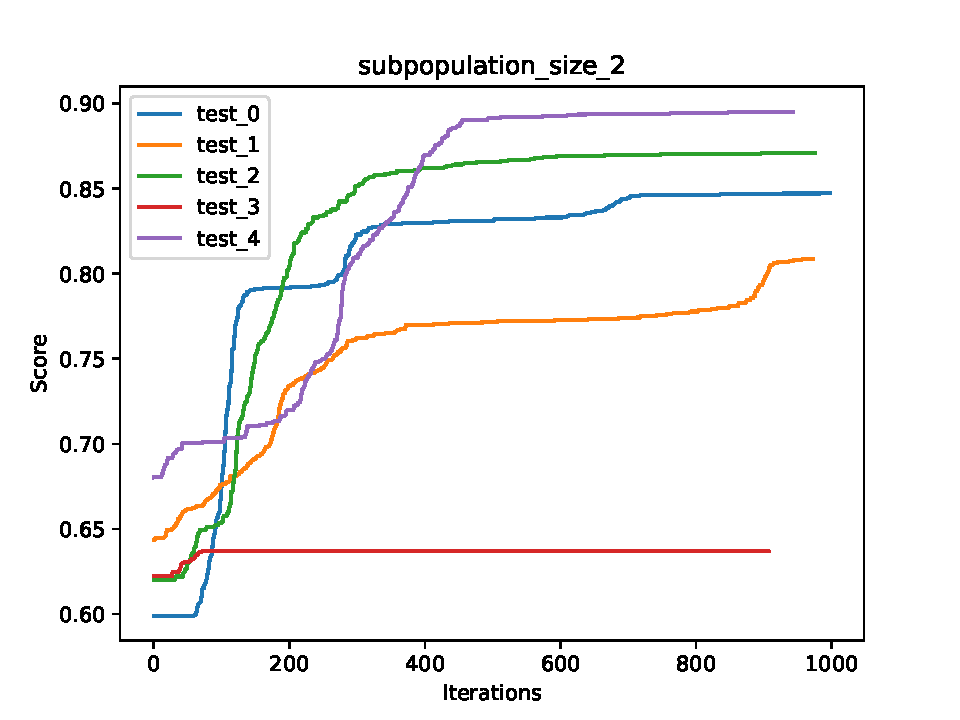
\includegraphics[width=\linewidth]{img/subpopulation_size_2.pdf}
        \caption{$\lambda$ = 200\%}
    \end{subfigure}
    \begin{subfigure}[b]{0.49\linewidth}
        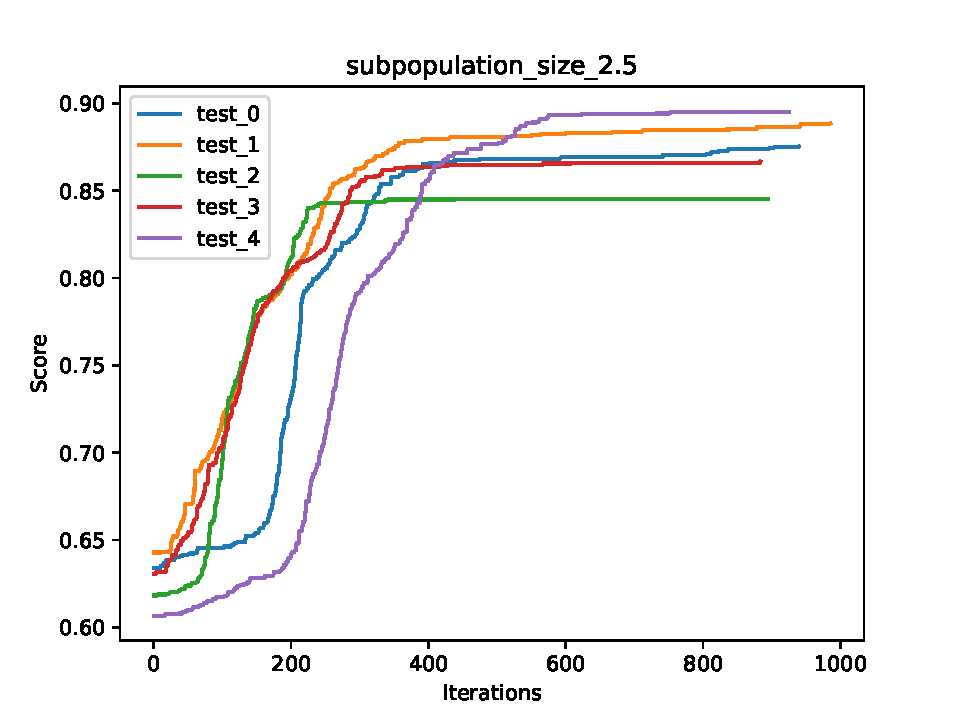
\includegraphics[width=\linewidth]{img/subpopulation_size_2.5.pdf}
        \caption{$\lambda$ = 250\%}
    \end{subfigure}
    \begin{subfigure}[b]{0.49\linewidth}
        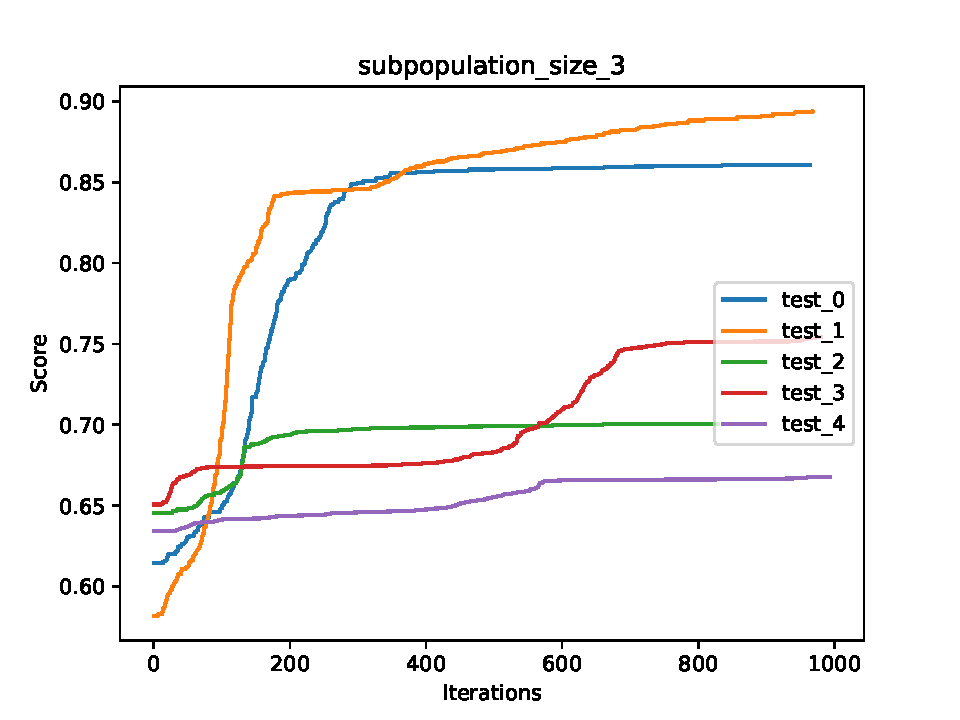
\includegraphics[width=\linewidth]{img/subpopulation_size_3.pdf}
        \caption{$\lambda$ = 300\%}
    \end{subfigure}
    \caption{Wielkość populacji $\lambda$}
    \label{fig:picking}
\end{figure}

\begin{table}[H]
    \centering
    \begin{tabular}{|c|c|c|}
    \hline
    Liczebność populacji $\lambda$  & Najlepszy osobnik & Średnio najlepszy osobnik \\ \hline
    110\%                           & 86\%              & 85\%                      \\ \hline
    130\%                           & 88\%              & 77\%                      \\ \hline
    150\%                           & 90\%              & 84\%                      \\ \hline
    200\%                           & 90\%              & 81\%                      \\ \hline
    250\%                           & 90\%              & 88\%                      \\ \hline
    300\%                           & 89\%              & 77\%                      \\ \hline
    \end{tabular}
    \caption{Wyniki testów liczebności populacji $\lambda$}
    \label{tab:crossing}
\end{table}

W przypadku wyników testu wielkości populacji $\lambda$ można powiedzieć, że zwiększenie wartości $\lambda$ do 250\% wartości $\mu$ daje najlepsze efekty. Dalsze zwiększanie wartości $\lambda$ powoduje spadek efektów końcowych.

\subsection*{Wpływ liczby prostokątów w osobniku}
Następny test został przeprowadzony dla następujących liczb prostokątów w osobniku: 10, 20, 50, 100, 200, 300. Wielkość populacji wynosiła 10, podpopulacji 15. Pozostałe parametry zostały niezmienione względem poprzedniego testu. 

\begin{table}[H]
    \centering
    \begin{tabular}{|c|c|c|}
    \hline
    Liczba prostokątów     & Najlepszy osobnik & Średnio najlepszy osobnik \\ \hline
    10                      & 86\%              & 84\%                      \\ \hline
    20                      & 86\%              & 78\%                      \\ \hline
    50                      & 85\%              & 76\%                      \\ \hline
    100                     & 74\%              & 72\%                      \\ \hline
    200                     & 75\%              & 74\%                      \\ \hline
    300                     & 75\%              & 74\%                      \\ \hline
    \end{tabular}
    \caption{Wyniki testów liczby prostokątów w osobniku}
    \label{tab:crossing}
\end{table}

\begin{figure}[H]
    \centering 
    \begin{subfigure}[b]{0.49\linewidth}
        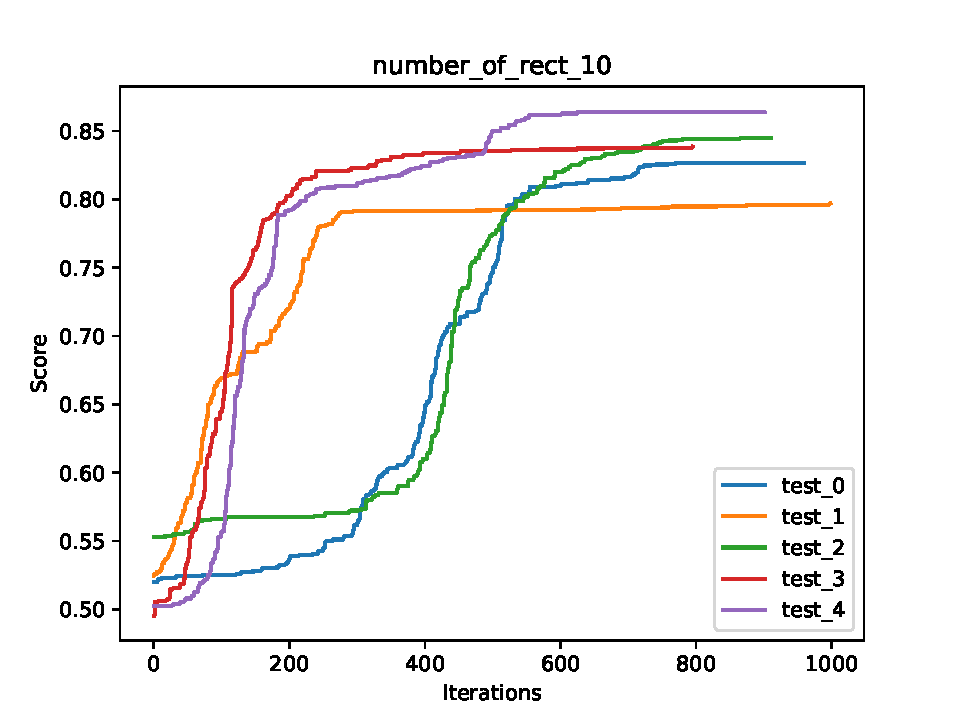
\includegraphics[width=\linewidth]{img/number_of_rect_10.pdf}
        \caption{10}
    \end{subfigure}
    \begin{subfigure}[b]{0.49\linewidth}
        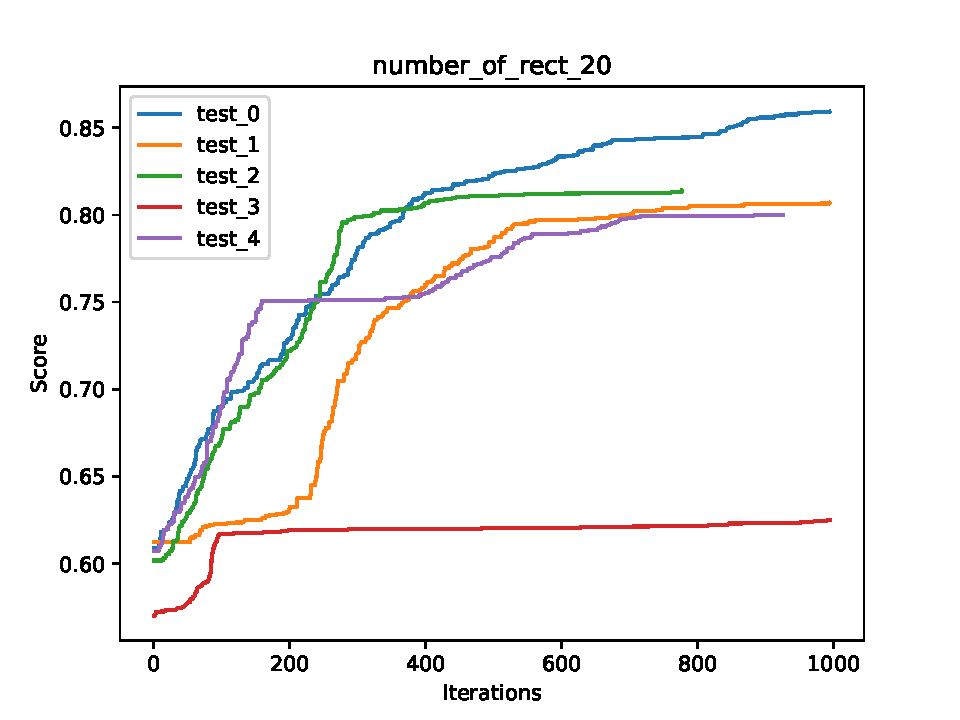
\includegraphics[width=\linewidth]{img/number_of_rect_20.pdf}
        \caption{20}
    \end{subfigure}
    \begin{subfigure}[b]{0.49\linewidth}
        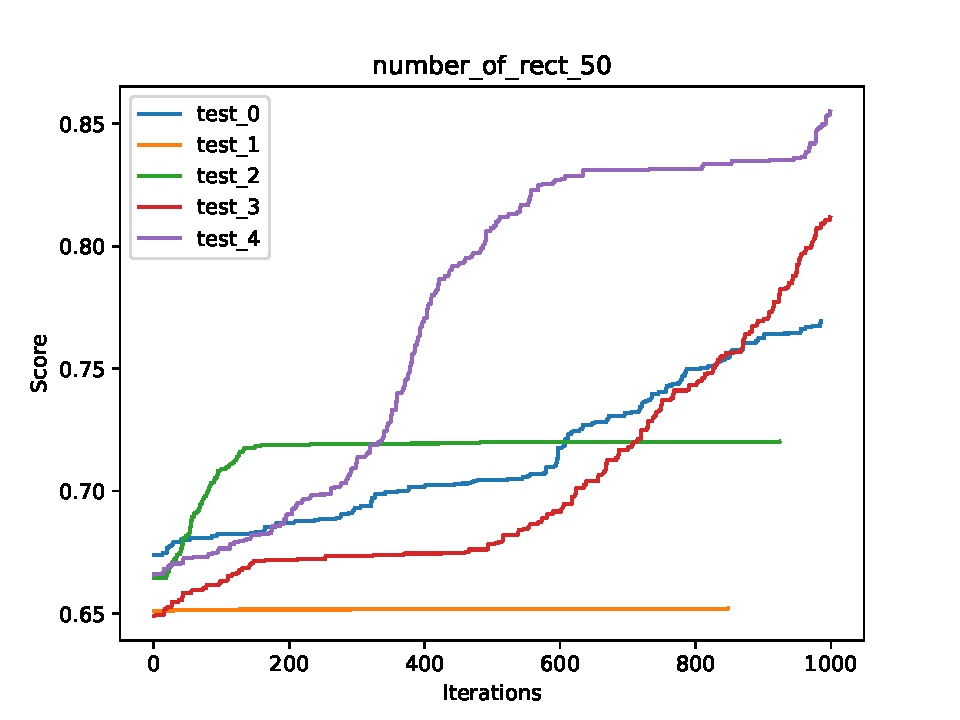
\includegraphics[width=\linewidth]{img/number_of_rect_50.pdf}
        \caption{50}
    \end{subfigure}
    \begin{subfigure}[b]{0.49\linewidth}
        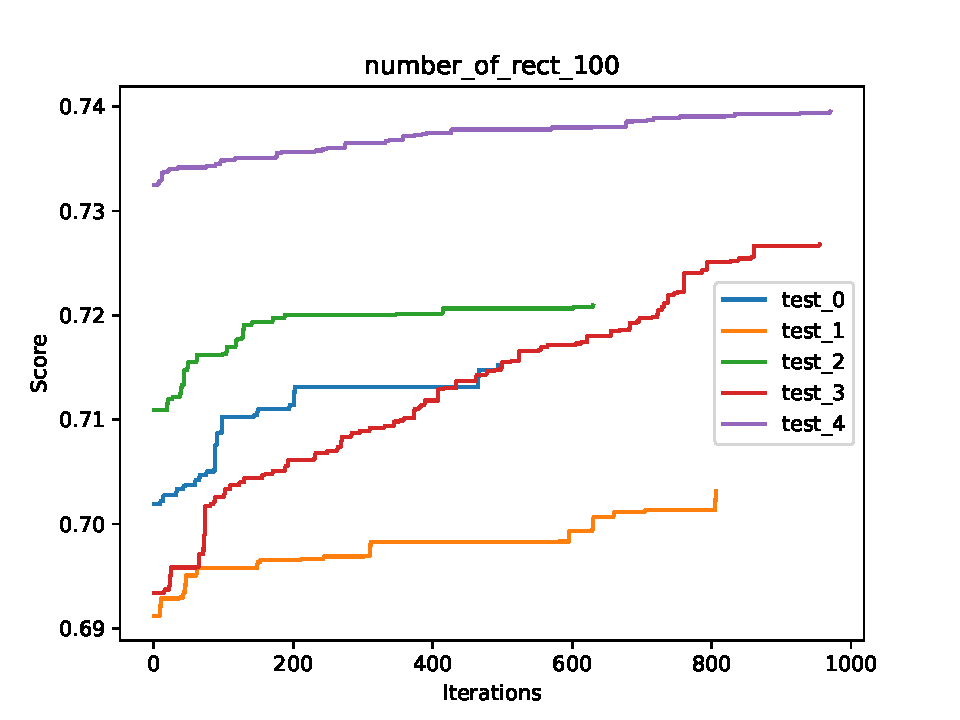
\includegraphics[width=\linewidth]{img/number_of_rect_100.pdf}
        \caption{100}
    \end{subfigure}
    \begin{subfigure}[b]{0.49\linewidth}
        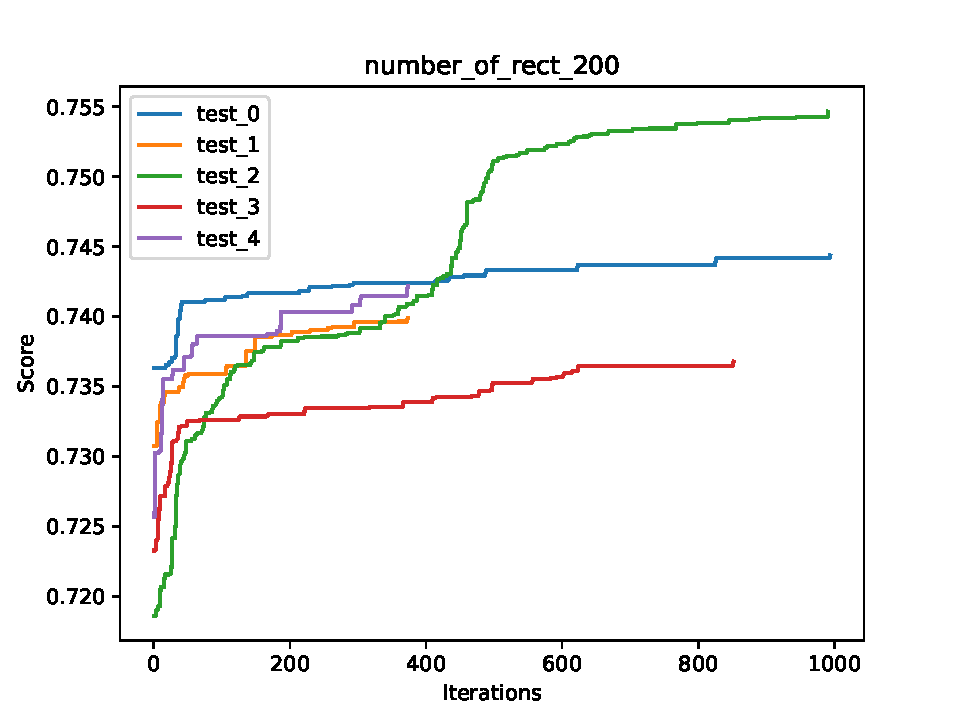
\includegraphics[width=\linewidth]{img/number_of_rect_200.pdf}
        \caption{200}
    \end{subfigure}
    \begin{subfigure}[b]{0.49\linewidth}
        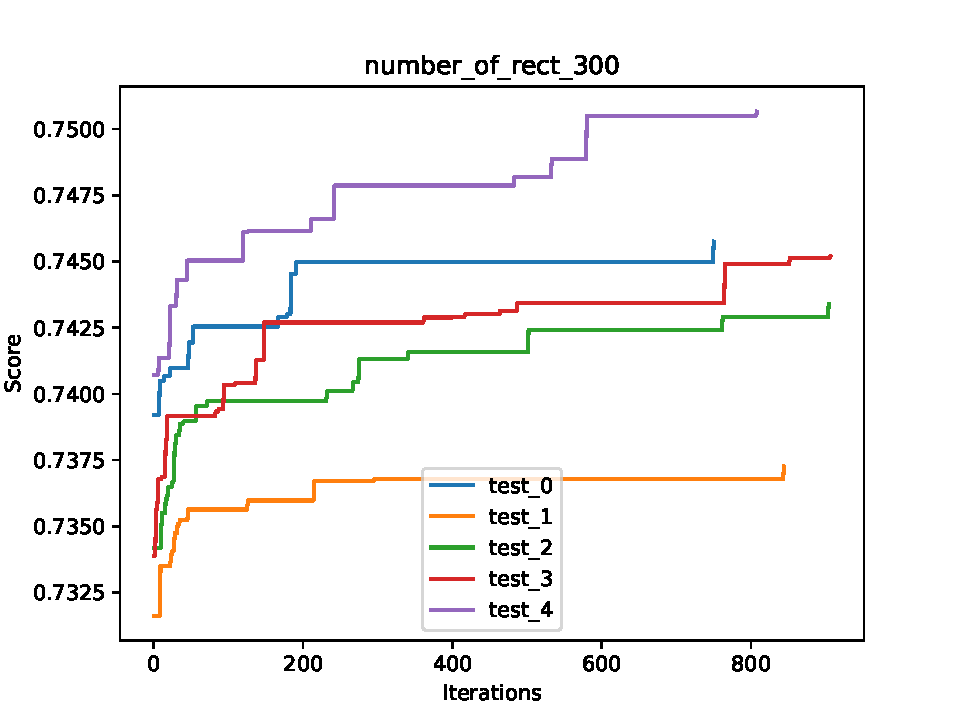
\includegraphics[width=\linewidth]{img/number_of_rect_300.pdf}
        \caption{300}
    \end{subfigure}
    \caption{Liczba prostokątów w osobniku}
    \label{fig:picking}
\end{figure}

W przypadku liczby prostokątów w osobniku można zauważyć, że w przeprowadzonym teście zwiększanie tej liczby zmniejsza dokładność odtworzenia zadanego obrazu. Wynika to z faktu, że zadany obraz składa się z 14 prostokątów o prawie jednolitych kolorach, więc algorytmowi łatwiej zbliżyć się do żądanej dokładności gdy używa mniejszej liczby prostokątów. Wynika to jedynie ze szegółowości obrazu wejściowego. By uzyskać najlepsze wyniki liczba prostokątów w osobniku powinna być zbliżona do liczby względnie jednolitych pól na obrazie.
\subsection*{Wpływ użytej strategii krzyżowania}
Dla populacji $\lambda$ - 20, populacji $\mu$ - 30 i liczbie 20 prostokątów w osobniku testy zostały przeprowadzone dla uśredniania i interpolacji.

\begin{figure}[h!]
    \centering 
    \begin{subfigure}[b]{0.49\linewidth}
        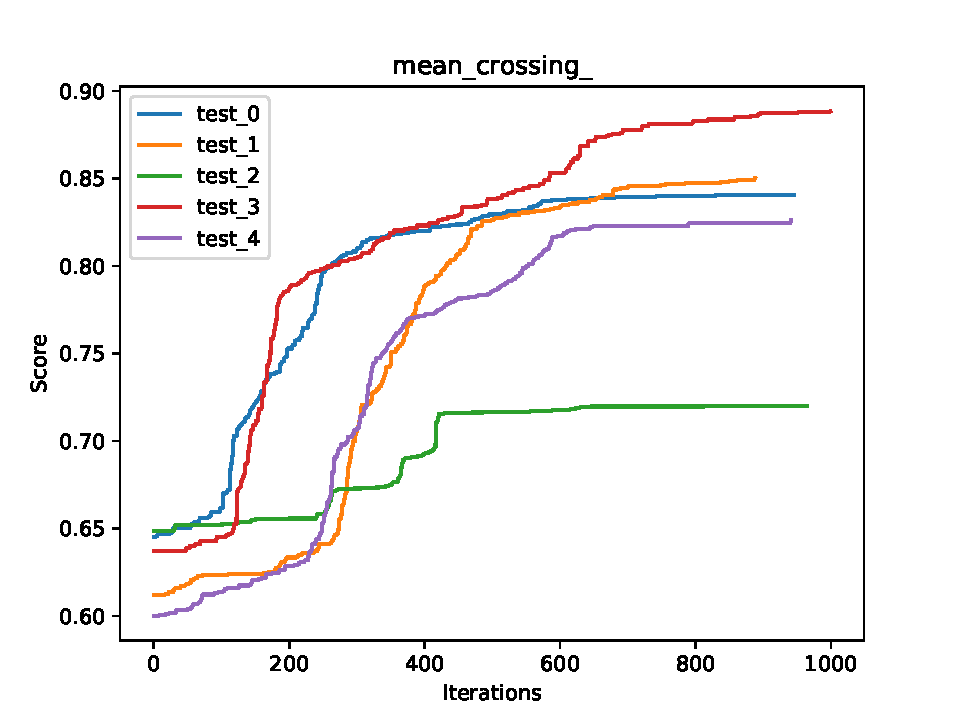
\includegraphics[width=\linewidth]{img/mean_crossing_.pdf}
        \caption{Uśrednianie}
    \end{subfigure}
    \begin{subfigure}[b]{0.49\linewidth}
        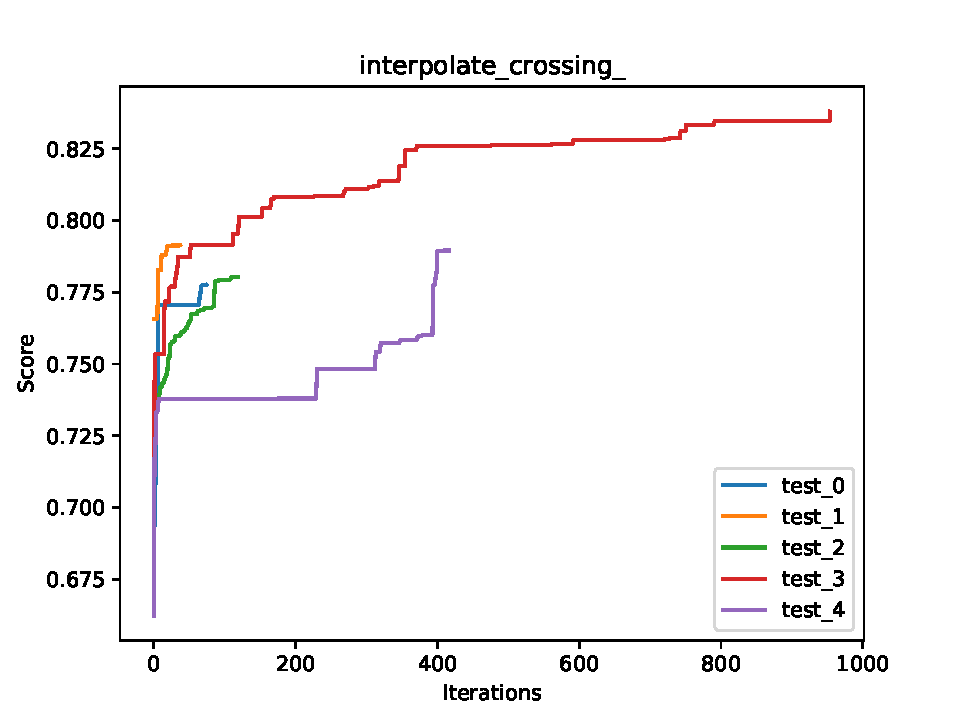
\includegraphics[width=\linewidth]{img/interpolate_crossing_.pdf}
        \caption{Interpolacja}
    \end{subfigure}
    \caption{Krzyżowanie}
    \label{fig:crossing}
\end{figure}

\begin{table}[H]
    \centering
    \begin{tabular}{|c|c|c|}
    \hline
    Metoda       & Najlepszy osobnik & Średnio najlepszy osobnik \\ \hline
    Uśrednianie  & 89\%              & 83\%                      \\ \hline
    Interpolacja & 83\%              & 79\%                      \\ \hline
    \end{tabular}
    \caption{Wyniki testów krzyżowania}
    \label{tab:crossing}
\end{table}

Dość dobrze widać, że w przypadku naszego problemu lepiej się sprawdza uśrednianie. Jeśli chodzi o interpolacje to warto zauważyć że wartości rosną bardzo szybko na początku, a potem zwykle zostają stałe lub niewiele się zmieniają. Może to być spowodowane, że algorytm dość szybko znajduje w naszym przypdaku osobnika z jednym lub kilkoma dużymi kwadrawtami, które potem ciężko rozmnożyć na lepsze osbniki. W przypadku uśredniania osbniki zmieniają się znacznie wolniej i taka sytuacja zachodzi rzadziej. 

\subsection*{Wpływ użytej strategii wybierania kolejnej populacji}
Dla populacji $\lambda$ - 20, populacji $\mu$ - 30 i liczbie 20 prostokątów w osobniku testy zostały przeprowadzone dla wyboru najlepszych, ruletki i metody rankingu.

\begin{figure}[H]
    \centering 
    \begin{subfigure}[b]{0.49\linewidth}
        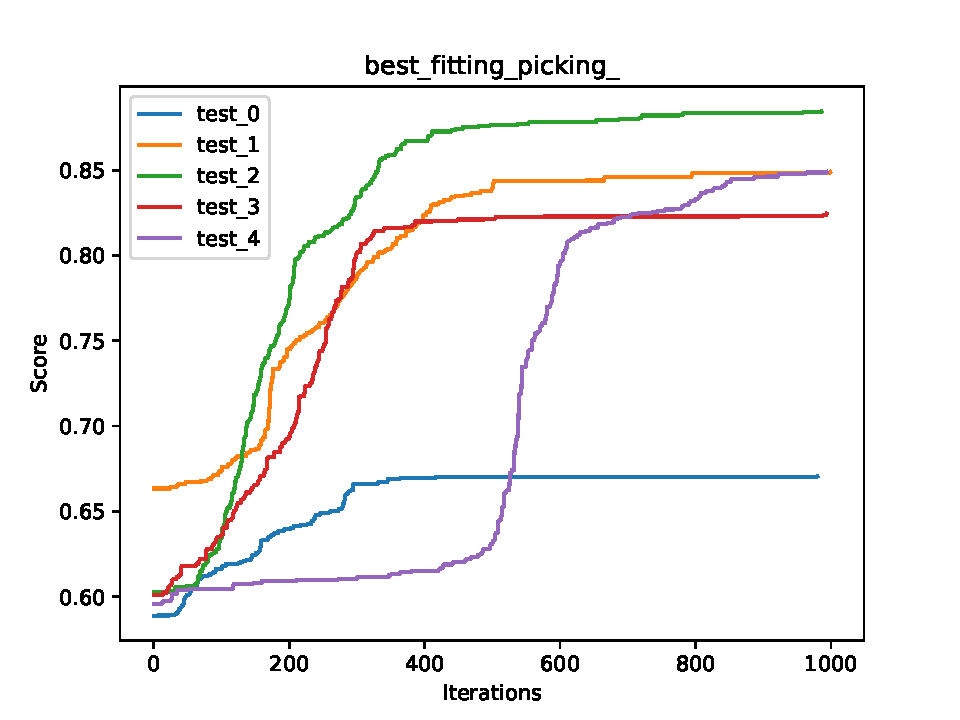
\includegraphics[width=\linewidth]{img/best_fitting_picking_.pdf}
        \caption{Wybór najlepszych}
    \end{subfigure}
    \begin{subfigure}[b]{0.49\linewidth}
        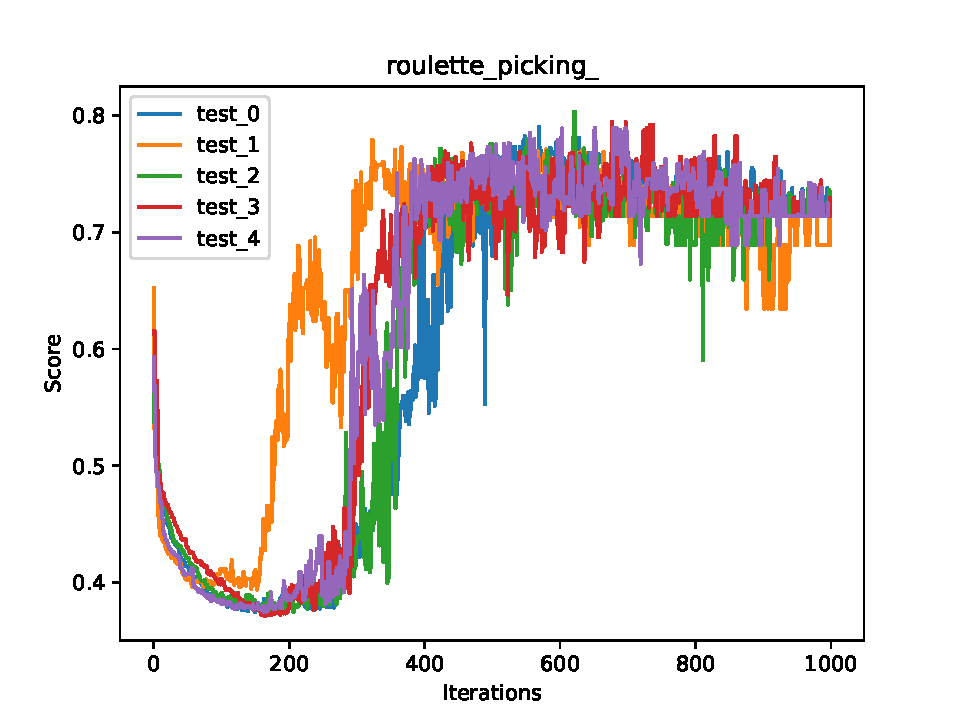
\includegraphics[width=\linewidth]{img/roulette_picking_.pdf}
        \caption{Ruletka}
    \end{subfigure}
    \begin{subfigure}[b]{0.49\linewidth}
        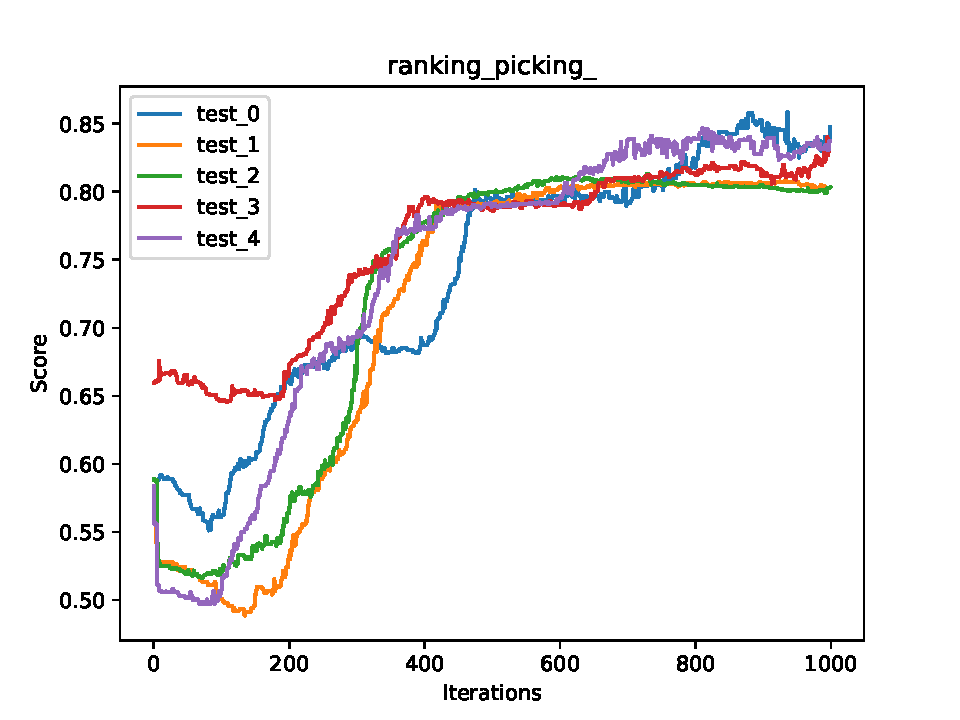
\includegraphics[width=\linewidth]{img/ranking_picking_.pdf}
        \caption{Ranking}
    \end{subfigure}
    \caption{Wybieranie}
    \label{fig:picking}
\end{figure}

\begin{table}[H]
    \centering
    \begin{tabular}{|c|c|c|}
    \hline
    Metoda       & Najlepszy osobnik & Średnio najlepszy osobnik \\ \hline
    Wybór najlepszych  & 88\%              & 82\%                      \\ \hline
    Ruletka      & 73\%              & 72\%                      \\ \hline
    Ranking      & 85\%              & 82\%                      \\ \hline
    \end{tabular}
    \caption{Wyniki testów wybierania}
    \label{tab:picking}
\end{table}
Ciężko stwierdzić, która metoda wybierania jest najlepsza, ale skłaniamy się do preferencji wyboru najlepszych lub przez ranking. Metoda ruletki wydaje się produkować najsłabsze rezultaty. Metoda wyboru najlepszych w późniejszych fazach traci mocno na efektywności. Metoda rankingu również w późniejszej fazie nieco zwalnia ale nie tak bardzo i wydaje się być dobrym rozwiązaniem dla naszego problemu.